\documentclass[11pt]{article}
\usepackage{url,graphicx,tabularx,array,amssymb,amsmath,color,setspace,amsthm}
%\usepackage{parskip}
\singlespacing
\pagenumbering{arabic}
\addtolength{\hoffset}{-1.5cm}
\addtolength{\textwidth}{3cm}
\addtolength{\voffset}{-1cm}
\addtolength{\textheight}{1.3cm}
\setlength{\parskip}{5pt}
%\setlength{\parindent}{0pt}
%\footskip=0pt
\newcommand{\sample}{\xleftarrow{\$}}
\usepackage{graphicx}
\graphicspath{ {images/} }
\newtheorem{theorem}{Theorem}

%\pagestyle{plain}
\title{Pseudo-Random Number Generators and their role in Computer Security}
\author{Vickram Rajendran, David Liu}
%\institute{}
\date{December 2016}
\begin{document}

\maketitle


\begin{abstract}
This paper details the use of pseudo-random numbers and their generation in computer security. Since there is no way to algorithmically create truly random numbers, the goal of pseudo-random number generators (PRNG's) is to create a sequence of numbers that cannot be distinguished from random numbers. PRNG's are used ubiquitously in computer science as a means to mimic randomness allowing for greater security in cryptography and other computer security.

We begin by dictating the various goals of pseudo-random number generation, their relation to quasi-random numbers, and their applications towards computer security. We discuss some of the earlier used PRNG's and their weaknesses against various attacks. After, we focus on the quality and speed of the currently prevailing PRNG's, and also examine the trade-off's involved in choosing a PRNG. We conclude with a discussion of the improvements and current research in PRNG's to prevent new attacks. 
\end{abstract}


\section{Introduction}

Random number generation pervades throughout Computer Science - every time we wish to shuffle our music, sample from a distribution, or even run electronic lotteries, we need to have some element of randomness in order to introduce unpredictability. However, creating true randomness is nearly impossible - the very fact that we are using a deterministic process to create these numbers means that the same inputs would create the same exact random numbers, thus getting rid of all randomness entirely. So, instead of trying to get true randomness, we attempt to have our random number generators create numbers that are indistinguishable from truly random numbers. The quality of a PRNG is thus naturally based on how computationally difficult it is to determine that the numbers generated from the PRNG were not random. 

There are two main methods of pseudo-random number generation, each of which can fulfill the quality checks for PRNG's. The first method is to have additional inputs, and use the variance in the inputs to create the pseudo-randomness. For example, a PRNG could include the temperature, wind speed, or other natural phenomena as some of its inputs. It would then be highly unlikely for the same inputs to ever repeat themselves, and by taking advantage of some "natural" randomness from the environment, the PRNG could create its pseudo-randomness. However, this clearly has some pitfalls, as it can be difficult to make sure that naturally random phenomena are being used, and it can also be very slow since the PRNG needs to gather enough outside data to be useful. 

The second method is having an algorithm that uses an initial seed to deterministically create a sequence of pseudo-random numbers. Though the algorithm will always present the same sequence when given the same initial seed, choosing different seeds will usually create wildly different sequences, and since only a single seed is necessary to create a slew of random numbers, it can be relatively fast. In practice, this is the method usually used for PRNG's.

If the goal of a PRNG is to create seemingly random numbers, then it is only natural the the goal of an attack on a PRNG is to prove that it is not random - this can be anything from guessing with high probability what the next generated number will be, to even determining a single bit of information that the next generated number will have. Both of the methods discussed above must be carefully implemented in order to maintain the quality of the PRNG, as there are many attacks for either method. However, current research and progress in PRNG's have sparked new innovation in the field, likely allowing for more creative and stronger PRNG's in the future that will be more resilient to these attacks. 

PRNG's are incredibly vital in Computer Security, and especially in cryptography. No encryption scheme with a deterministic encryption algorithm can be semantically secure, and so PRNG's are necessary in order to have a semantically secure cryptographic system. PRNG's are also used in message authentication codes, some hash algorithms, and many other topics in computer security - Thus, these cryptographically secure PRNG's must be of the highest quality in order to prevent attacks from compromising even the slightest bits of security. 


\subsection{Related Work}

Closely related work to Pseudo-Random numbers are work in the low-discrepancy sequences (quasi-random numbers). A sequence is considered to have low discrepancy if given an arbitrary set of points, the proportion of points from the sequence in that set is close to proportional to the volume of the initial set. These types of numbers are not truly random or pseudo-random, in that they do not necessarily have a seemingly random distribution, but they can be highly useful in order to mimic uniform distribution of a sequence. 

Quasi-random numbers can be more useful than pseudo-random numbers in a plethora of ways. For example, consider the standard implementation of the Monte-Carlo integration method: $$\int_a^b f(x) \approx \frac{1}{N}\sum_{i = 1}^N f(x_i)$$ where each $x_i \in [a, b]$, and each $x_i$ is generated from a PRNG. Unfortunately, a PRNG would almost never cover the interval $[a, b]$  uniformly - since each number should have an equal chance of being picked, regardless of how close it is to previously picked numbers, the PRNG might inadvertantly bias certain parts of the interval of integration. However, quasi-random numbers for the $x_i$ would remove this problem, as the low-discrepancy of the numbers would ensure that the interval is almost evenly covered \cite{quasi}.  Thus the quasi-Monte Carlo integration method is far superior to its counterpart, as it takes into account a more uniform distribution of the domain of integration. 

Though quasi-random numbers have their uses, their uniformity is an immense obstacle to their use in computer security - see Figure $1$ to see how easily distinguishable they are from a quality PRNG. Some research is currently going on in attacks that attempt to reduce PRNG's to quasi-random numbers, but no real attacks have come from this connection as of yet \cite{quasi}. 

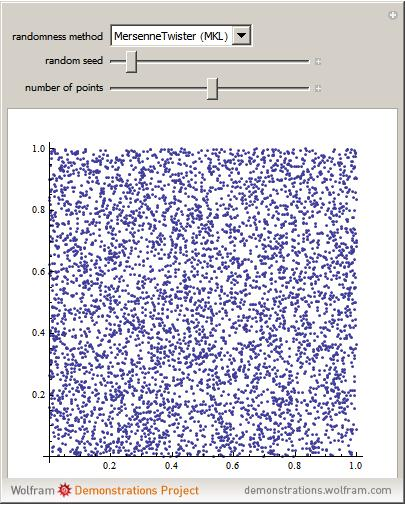
\includegraphics[scale=.5]{MersenneTwister}
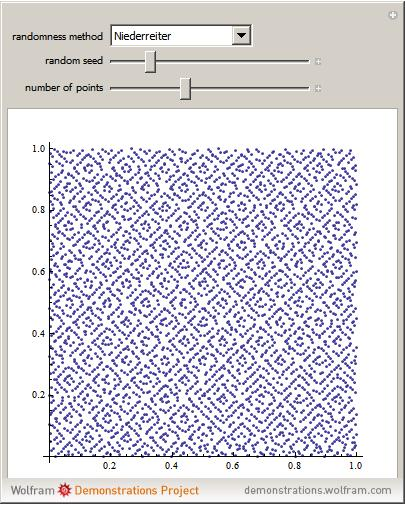
\includegraphics[scale=.5]{Niederreiter}

Figure 1: This is a large amounts of points from both a PRNG and a Quasi-Random number generator. The Mersenne Twister (Left) is a PRNG, and clearly seems to be random points, while the Niederreiter (Right) is quasi-random and has clear patterns in distribution. \cite{Mersenne}
\section{Background and Definitions}
Unless otherwise stated, a PRNG will refer to the second sense of PRNG's - in that there is an initial seed and the random numbers are chosen from the sequence that this seed generates.


Throughout the paper, we will use "hard" to mean computationally difficult. More specifically, something is hard if it cannot be accomplished computationally within a polynomial amount of time. 

The "period" of a pseudo-random number generator will be used in regards to the second sense of PRNG's. Given an arbitrary seed, the "period" is the amount of numbers generated before the sequence has a repeat.

We will use the terminology of "initializing a PRNG" to reference starting the PRNG with a seed state, and using the values of the sequence created by that seed. 

A linear congruential generator (LCG) is a PRNG that is based off of a linear recurrence with modular arithmetic. This means that the succeeding members in the sequence are based off of some sort of linear relation between the preceeding member of the sequence: If $X_n$ was a sequence created by an LCG, then $$X_n = (aX_{n-1} + b)  \mod m$$ where $a, b, m$ are all integers and $m > X_0$ where $X_0$ is the seed. 

A "Cryptographically secure" PRNG will be explicitly defined as follows: Let $F$ be a PRNG, and let $G$ be a truly random function. Given any adversary $A$ that does not know the seed that initialized the PRNG $F$, then we define the advantage of $A$ on $F$ to be $Adv_F(A) = Pr[A(F) = 1] - Pr[A(G) = 1]$, where $Pr[A(H) = 1]$ means the probability that the adversary $A$ outputs a bit $1$ when presented with the function $H$. $F$ is cryptographically secure if $Adv_F(A) <<<< 1$. 

"Entropy" will be used to refer to the true randomness that naturally occurs in the world - for example, atmospheric noise, quantum/electrical phenomena, the cosmic microwave background, etc. 


\section{Weaknesses in Early PRNGs}
\subsection{The Diehard Tests}
George Marsaglia, one of the greatest minds in Random number generation, created a series of tests in order to measure how random certain PRNG's were suppposed to be. These "Diehard Tests", published in 1995, were the hallmark of any good PRNG, and the tests also invalidated many of the existing PRNGs at the time. We will use these tests to show that several of the early PRNG's were not cryptographically secure. The Diehard tests will be detailed in the appendix. 

\subsection{Middle Square Method (Von Neumann)}
In 1946, John Von Neumann suggested one of the first computational algorithms to be used for a PRNG. The algorithm is as follows: \newline
Let $D$ be the amount of digits for each random number, and let $S_0$ be a seed with $D$ digits. Take the middle $D$ digits of $S_0^2$, and let this be the next random number.

It is clear that this PRNG is not cryptographically secure, as we can quickly predict the next values of the PRNG. Also, we know that some seeds will have incredibly short periods (consider $S_0 = 0000$, which immediately repeats). A simple adversary that looks at two consecutive values would be able to tell without reasonable doubt that the Middle Square Method was used. This method also, naturally, fails several of the Diehard tests. While this method might not be the most secure, it was useful at the time as PRNG's weren't prevalent in cryptography and were not held to such a high standard. Regardless, something a bit stronger would be needed in the future, which led to Linear Generators.
\subsection{Linear Congruential Generators}
Recall that an LCG is a PRNG initialized with $X_0$ defined as follows: $$X_n = (aX_{n-1} + c) \mod m$$ LCG's provided a myriad of benefits that their predecessors ignored. Firstly, since they were based off of modular arithmetic, they were incredibly fast and did not take much space. Also, it was relatively easy to increase the period of an LCG, as all we would have to do is increase the value of $m$, the modulus \cite{Well}. In fact, the conditions that allow an LCG a full period are fully dictated in the following theorem: 
%http://chagall.med.cornell.edu/BioinfoCourse/PDFs/Lecture4/random_number_generator.pdf 
\paragraph{The Hull-Dobell theorem \cite{HD}:} 
An LCG has a full period for all seed values if and only if: 
\newline
1. $m, c$ are relatively prime. \newline
2. $a - 1$ is divisible by all prime factors of $m$. \newline
3. $a - 1$ is divisible by $4$ if $m$ is divisible by $4$. 

Unfortunately, having a full period does not necessarily make a PRNG secure. All LCG's, by virtue of construction, have patterns in their sequences through autocorrelation. This means that the LCG has correlations with itself when the sequence has grown large enough. The amount of elements necessary to determine this pattern is not large enough to prevent autocorrelation from being a large problem with LCG's. 

This autocorrelation can be seen through the following analysis. Since the LCG is by definition linear, we have a lot of information about the distribution of the elements. Linearity means that in certain dimensions, we can confine the sequence of the LCG onto a certain amount of hyperplanes. The results are summarized in the following theorem:

\paragraph{Marsaglia's Theorem: \cite{Marsaglia}}
If $n$ points were constructed from an $LCG$, then the points lie on at most $(n!m)$ hyperplanes in $\mathbb{R}^n.$

Once again, new methods became necessary in order to achieve high quality randomness. 
\subsection{Linear Recurrences}
Once algorithms moved past LCG's and into allowing Linear recurrences in general, the algorithms became more robust. As long as the output was perturbed slightly, autocorrelation didn't appear to be a problem, and three PRNG's became prevalent as the best algorithms at the time: The xorshift algorithm, the Mersenne Twister, and the WELL algorithms. 
\paragraph{xorshift} 
The xorshift family, created by George Marsaglia in 2003 worked by xor'ing a number with a bit-shifted version of itself. This made them incredibly fast, as xor's are not computationally expensive to do, and yet they still seemed to be incredibly pseudo-random. Plain xorshift algorithms failed a few Diehard tests, but when Marsaglia added a non-linear perturbation to the output, creating xorshift+, they became relatively secure. 

However, these algorithms are still not cryptographically secure. It is possible to reconstruct the seed when given multiple outputs of an xorshift generator, which means that one would be able to still predict the next value from an xorshift. Using xorshift+ algorithms, like xorshift128+ helps, but not enough to render the algorithm cryptographically secure. However, the speed and moderate quality of randomness makes xorshift a popular choice for PRNG's that don't require higher quality security. 

The insecurity of xorshift was also exploited in HackMIT's challenge problems for this year. MIT regularly hosts challenge problems, of which the first fifty solvers get free entry to their hackathon. Their final problem this year was predicting the next output of their random number generator, which used xorshift128+ \cite{hackMIT}. The solvers had to get several values of the sequence (which would be truncated due to browser's using mantissa's) created by the seed, and then use a satisfiability solver such as Z3 in order to reconstruct what the seed had to be in order to get these truncated values. Finally, the students would have to step through the xorshift128+ process to find out what the RNG would give out, and then predict it. This is a clear and clever example of how insecure xorshift128 is, even in its nonlinear form, when given some of the output values of the sequence.  
\paragraph{Mersenne Twister}
The Mersenne Twister, created in 1997, was the most prevalent PRNG of the time, and is still widely used as a PRNG that does not need to be cryptographically secure. Its prowess comes from its period being a Mersenne Prime (the standard implementation has a period of $2^{19937}-1$), and the fact that it has a guaranteed random distribution for large numbers. It also passes all of the Diehard tests, and is considered to be one of the best PRNG's that is not cryptographically secure \cite{Mers}.  Unfortunately, this algorithm takes up a lot of space, and does not run nearly as fast as xorshift. Also, after $624$ iterations, all future values of the Twister can be predicted, which means that it is not cryptographically secure \cite{Well}. Finally, the complexity of the algorithm was difficult to follow and took some time in actually constructing the pseudo-random number - see Figure 2. 
\paragraph{WELL} The WELL (Well Equidistributed Long-period Linear) family of PRNG's were meant to be an improvement on the logistical aspects of the Mersenne Twister. No one had any complaints about the quality of the Twister's randomness, but the storage space necessary and the complexity of the algorithm made it unattractive for certain purposes. The WELL algorithms lowered the storage space and made several quality of life improvements to the Mersenne Twister, at the cost of some advantages like the guaranteed strongly random distribution \cite{Well}. 

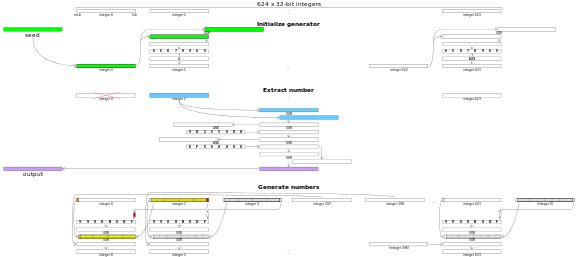
\includegraphics[scale = .85]{MT_v}
Figure 2: A visualization of the Mersenne Twister's algorithm. 
\section{Cryptographically Secure PRNGs}
There are three main ways to prove that a PRNG is cryptographically secure. 

The first way is to base the PRNG on a cryptographic primitive, such as a cipher. Then one can reduce the PRNG to solving the cipher, which is known to be hard.

The second way is to reduce the PRNG to a problem that is known to be hard. That is, an adversary that has non-negligible advantage towards the PRNG could be used to construct a solution to a hard problem. Then if we believe that the problem is truly hard, it would be computationally infeasible for any adversary to gain advantage over the PRNG. The classic problem to reduce to is integer factorization, as this problem is believed to be hard, and many of the cryptographically secure PRNG's will reduce to this.

The final way is to have the PRNG to be cryptographically secure by construction, in that it is specifically designed with cryptography in mind. We examine examples of all three. 
\subsection{Cipher based}
\paragraph{Stream ciphers}
Stream ciphers are based off the idea of the one-time pad - this is the idea that if you have a random key as long as your message, then you can encrypt each bit of the message with the corresponding random bit of the key, which is completely secure since each bit is randomly changed. A stream-cipher uses the PRNG to create the random key as long as the message, and then combines it with the plaintext to encrypt the message. This is considered a stateful algorithm, since the stream is constantly shifting. Not all stream ciphers are cryptographically secure - it depends on the quality of the PRNG used to create the stream. However, if the PRNG satisfies the statistical tests, then this can be used as a cryptographically secure PRNG.
\paragraph{Block Ciphers} We have gone over these extensively in class, and we know that there exist cryptographically secure Block Ciphers like DES and AES (with sufficient bit complexity). We can use these to construct PRNG's, for example by running the block cipher in counter mode. Basically, first choose a random key for the block cipher, and then let $BC(k, 0)$ be the seed value for the PRNG, and let $BC(k, n) = X_n$ for the remaining values of the PRNG. Clearly this is cryptographically secure if the block cipher is secure. 
\subsection{Problem Based}
Many of these algorithms are far more inefficient to use since they require a lot of machinery in order to make them reduce to the certain math problems.
\paragraph{Blum Blum Shub \cite{BBS}} The Blum Blum Shub algorithm works as follows. Given a seed $X_0$, we have $$X_n = X_{n-1}^2 \mod M$$ where $M$ is a very large semi-prime that is hard to factor. There exists a really complicated proof that shows that this is related to integer factorization, and since integer factorization is considered to be a hard problem, this algorithm is a cryptographically secure PRNG \cite{BBS}. However, squaring numbers is a lot of space and can be difficult computationally, especially with how large these numbers can get, so this algorithm is highly inefficient and impractical to use. 
\paragraph{Blum-Micali} This algorithm works as follows: Given a seed $X_0$, let $$X_n = g^{X_i} \mod p$$ with $g$ a number that gives all values mod $p$ when exponentiated, and $p$ a very large prime. Then this algorithm will be secure based on the discrete logarithm problem, which we also believe to be hard. Once again, using this over and over again can be very inefficient, and thus this algorithm is almost never used in PRNG's.
\subsection{Constructive}
These types of algorithms are the most creative, and also the algorithms that are currently going through the most active research. 
\paragraph{Yarrow}
The Yarrow algorithm has four main components that is used in order to make it resistant to any form of attacks \cite{Yarrow}. The first component accumulates entropy from various sources - these sources can be physical sources like atmospheric noise or quantum phenomena. The amount of entropy collected will directly relate to how drastic of a change there will be to the seed. The second component re initializes the key with different values based on how much entropy has been accumulated by the first component. The third mechanism is the actual PRNG which generates pseudo-random numbers based on the key, and the final component is a control mechanism that tells when the key needs to be re-seeded \cite{Yarrow}. Yarrow was designed to be a new cryptographic primitive - basically, this means that it was meant to be a building block for other cryptographic results. Also, note that the other cryptographically secure algorithms were proven secure by reducing them to an existing cryptographic primitive that was known to be hard - this is not the case with Yarrow. It was designed to be cryptographically secure, just like the next algorithm.
\paragraph{Fortuna}
As if Yarrow was not good enough, it has quickly been replaced with Fortuna, the currently used PRNG by python cryptography and in linux's dev/random \cite{Fortuna}. Fortuna is very similar to Yarrow, but it differs in its entropy accumulation and its seeding mechanism. In Yarrow, the entropy is accumulated into two separate pools - one for "fast" reseeding, and one for "slow" reseeding. Fortuna, on the other hand, uses many more pools, and uses each pool with a certain probability to reseed. Thus the first pool collects small entropy, but reseeds frequently, but the 6th pool will collect a large amount of entropy, but reseed infrequently \cite{Fortuna}. By implementing a larger amount of pools, an attacker is unlikely to corrupt all of the pools and thereby compromise the cryptographic security of the algorithm. Fortuna's use of $32$ pools makes this inviable, and makes Fortuna one of the most secure algorithms on the planet. 
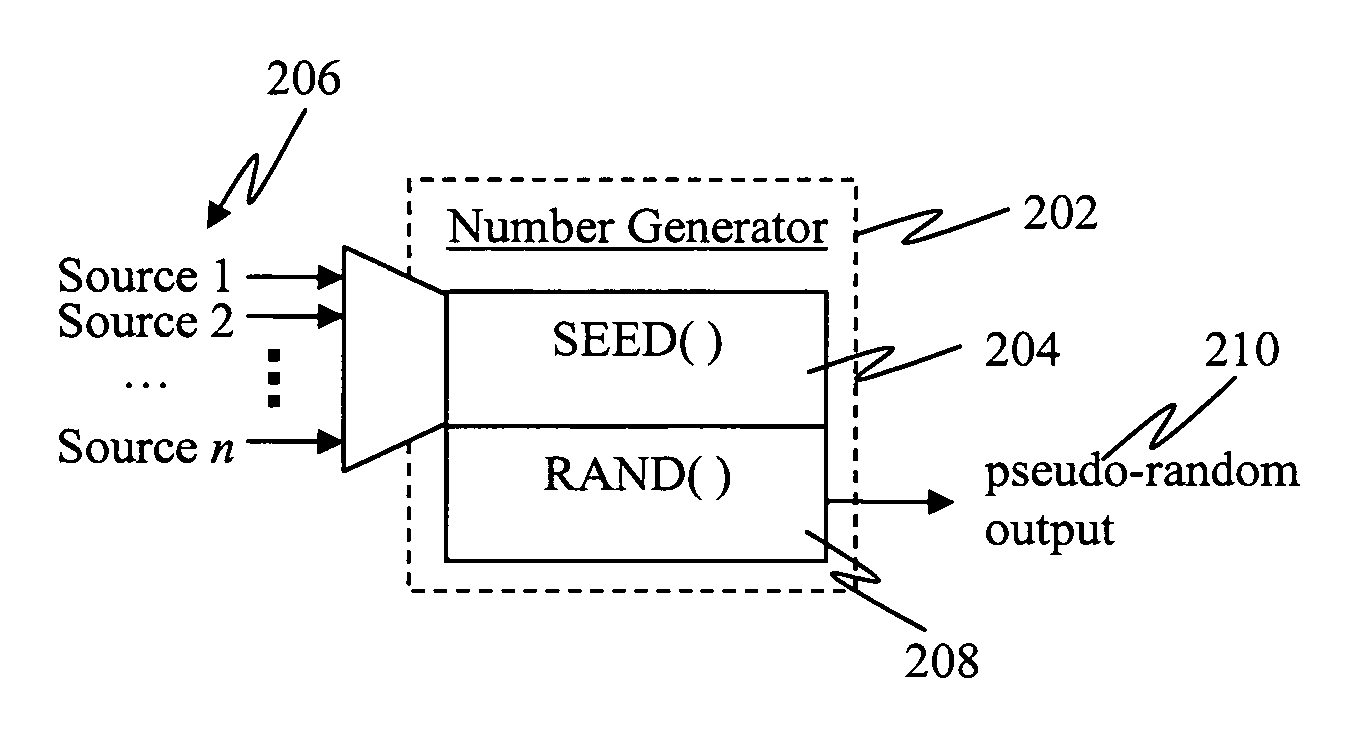
\includegraphics[scale = .3]{fortuna} \newline
Figure 3: Yarrow and Fortuna's basic implementation \cite{patent}. 
\section{Conclusion}
Pseudo-random number generation has improved immensely in the past fifty years, and we can expect to see this progress only continue. The quest to find the ultimate PRNG has not subsided - if anything, the development of Fortuna and other PRNGs as cryptographic primitives have only sparked even more innovation in this field. 

As recently as 2005, Gregory Gordon Rose, Alexander Gantman, Lu Xiao filed a patent for an improvement on Fortuna's use of block ciphers in counter mode and its use of cryptographic hashes \cite{patent}. Non-uniform generators have also been undergoing examination to have pseudo-random sampling from certain non-uniform probability distributions. Evolutionary algorithms are also undergoing research in order to create pseudo-random numbers - these would be algorithms that implement some sort of artificial intelligence in order to get cryptographically secure pseudo-random numbers. An evolutionary algorithm has already been created by the National Institute of Standards and Technology statistical test suite, and more are sure to follow. 

However, as time goes on, new mathematical concepts and new computer science ideas will be found, which may render our current PRNG's insecure - if that becomes true, it will be necessary for us to find better PRNG's. The constant cycle of PRNG, and then attack on PRNG will continue as it has for the past fifty years. Whenever there is a PRNG, there will be people trying to attack it, and whenever there is a successful attack, there will be people creating the next secure PRNG. This circle of innovation can only lead to amazing progress in the field of Pseudo-random number generation. 


\bibliographystyle{abbrv}
\bibliography{thebib}


\appendix
\section{Appendices}
\section{The Diehard Tests}
\paragraph{Birthday Spacings:}
Use the PRNG to find random points on a large interval- the spacing between these points should be exponentially distributed, as the birthday paradox tells us.
\paragraph{Overlapping Permutations:}
Use the PRNG to find several sequences with the same five consecutive numbers. The $5! = 120$ possible orderings should occur with equal probability (up to sampling). 
\paragraph{Ranks of Matrices} 
Select some of the bits from some random numbers to form a matrix with $0$'s and $1$'s, and count the rank of this matrix. It should not be the same for various random numbers.
\paragraph{Monkey Tests}
See if there are any repeats in the sequence, or any overlapping subsequences in the sequence. 
\paragraph{Count the 1's}
Count the amount of $1$ bits in some bytes. See how many times certain distributions of the $1$'s occur, and make sure that there is no pattern.
\paragraph{Parking Lot Test}
Use the PRNG to randomly place unit circles somewhere in an 100 x 100 square. See the distribution of circles that do not overlap any other circle after 12,000 tries, it should be normal.
\paragraph{Minimum Distance}
Place $8000$ points in a 10,000 x 10,000 grid, find the minimum distance between pairs. The square of this should be exponentially distributed.
\paragraph{Random Spheres} Do the same thing as the parking lot test, but with spheres in a cube instead of circles in a square. 
\paragraph{Squeeze}
Multiply $2^{31}$ by random numbers until it gets to $1$. The amount of numbers needed to do this should follow a distribution.
\paragraph{Overlapping Sums}
Add sequences of $100$ randomly generated numbers. The sums should be normally distributed.
\paragraph{Runs}
Make random sequences, count the runs that are ascending and the ones that are descending. These should also follow a certain distribution.
\paragraph{Craps}
Play lots of craps games, the wins and number of throws should follow a certain distribution. 
\end{document} 